\section{Čech 上同调}
\sourcepage{519--520}
至今研究了单纯和奇异两种同调、上同调理论。还有其他理论，其中最著名的是 Čech 理论，尤其在上同调方面表现良好。本节构造其上同调群，证明在可三角剖分空间上与单纯群一致，并给出与奇异群不同的空间。下一节将用它证明推广的 Alexander 对偶。

\entry{定义}{8.13.1}\emph{有向集}是一个带关系 $<$ 的集合 $J$，满足：(1) $\alpha<\alpha$；(2) 若 $\alpha<\beta<\gamma$，则 $\alpha<\gamma$；(3) 任意两个元素都有共同上界，即存在 $\delta$ 使 $\alpha<\delta$、$\beta<\delta$。这里的记号 $<$ 不要求反自反。

\entry{例}{8.13.2}任何全序集在关系 $\le$ 下都是有向集。

\entry{例}{8.13.3}空间所有开覆盖组成有向集：令 $\mathcal A<\mathcal B$ 表示 $\mathcal B$ 加细 $\mathcal A$，即后者每个成员包含于前者某个成员。自反性、传递性显然；两覆盖所有交集 $A\cap B$ 组成共同加细。

\entry{定义}{8.13.4}以有向集 $J$ 为指标的阿贝尔群\emph{直系统}，由群 $G_\alpha$ 及对每个 $\alpha<\beta$ 定义的同态 $f_{\alpha\beta}:G_\alpha\to G_\beta$ 组成，满足
\[f_{\alpha\alpha}=i,\qquad f_{\beta\gamma}f_{\alpha\beta}=f_{\alpha\gamma}.\]

\entry{定义}{8.13.5}在各群的不交并上，令 $g_\alpha\sim g_\beta$，当且仅当存在共同上界 $\delta$，使 $f_{\alpha\delta}(g_\alpha)=f_{\beta\delta}(g_\beta)$。等价类集合称为\emph{直极限}，记为 $\varinjlim_{\alpha\in J}G_\alpha$。其加法定义为
\[\{g_\alpha\}+\{g_\beta\}=\{f_{\alpha\delta}(g_\alpha)+f_{\beta\delta}(g_\beta)\}.\]
容易检验运算定义良好，并使其成为阿贝尔群。若全部结构映射为同构，极限同构于任一群；若对每个 $\alpha$ 都存在 $\beta>\alpha$ 使 $f_{\alpha\beta}=0$，极限为零，特别地结构映射全为零时如此。

\entry{定义}{8.13.6}两个直系统之间的\emph{映射}，包括保序映射 $\varphi:J\to K$ 与同态 $\varphi_\alpha:G_\alpha\to H_{\varphi(\alpha)}$，使结构映射组成的方块交换。它诱导直极限同态
\[\Phi_\to:\varinjlim_JG_\alpha\to\varinjlim_KH_\gamma,\qquad
\{g_\alpha\}\mapsto\{\varphi_\alpha(g_\alpha)\}.\]

\sourcepage{521--522}
\entry{例}{8.13.7}若对固定群 $H$ 有相容同态 $\varphi_\alpha:G_\alpha\to H$，即 $\varphi_\beta f_{\alpha\beta}=\varphi_\alpha$，则诱导 $\varinjlim G_\alpha\to H$。这就是目标直系统只含一个群的特殊情形。

\entry{例}{8.13.8}群序列 $G_1\xrightarrow{f_1}G_2\xrightarrow{f_2}\cdots$ 构成直系统，令 $f_{mn}=f_{n-1}\cdots f_m$。若所有群为 $\Z$，各映射为乘以 $2$，则直极限为二进有理数的加法群
\[\{m/2^r:m\in\Z,\ r\ge0\}.\]
定义 $\varphi_n(m)=m/2^n$，它们相容，所诱导同态容易检验既单又满。

\entry{定义}{8.13.9}若对每个 $\alpha\in J$，都存在 $\delta\in J_0$ 使 $\alpha<\delta$，则称子集 $J_0$ 在 $J$ 中\emph{共尾}。

\entry{引理}{8.13.10}共尾子集本身为有向集，且包含诱导 $\varinjlim_{J_0}G_\alpha\cong\varinjlim_JG_\alpha$。

\textbf{证明：}两个 $J_0$ 中元素先在 $J$ 中取上界，再取 $J_0$ 中更大的元素，即得共同上界。诱导同态满，因为每个元素可向前映到 $J_0$ 的某个群。若 $g_\alpha$（$\alpha\in J_0$）在大极限中为零，则在某个 $G_\delta$ 中像为零；再选 $\epsilon\in J_0$ 大于 $\delta$，其像在 $G_\epsilon$ 中也为零，所以在小极限中已为零。\hfill$\square$

\entry{定义}{8.13.11}对空间的一族子集 $\mathcal A$，定义抽象复形\emph{神经} $N(\mathcal A)$：顶点为该族成员，有限子族组成单形，当且仅当其交非空。

若 $\mathcal B$ 加细 $\mathcal A$，为每个 $B$ 选取包含它的 $g(B)\in\mathcal A$，得到单纯映射 $g:N(\mathcal B)\to N(\mathcal A)$。不同选择彼此邻接，因为
\[\bigcap B_i\subset\bigcap\bigl(g(B_i)\cap g'(B_i)\bigr),\]
所以诱导相同同调和上同调同态。

\entry{定义}{8.13.12}这些唯一确定的同态称为\emph{加细诱导的同态}：
\[g_*:H_k(N(\mathcal B);G)\to H_k(N(\mathcal A);G),\qquad
g^*:H^k(N(\mathcal A);G)\to H^k(N(\mathcal B);G).\]

\sourcepage{523--524}
\entry{定义}{8.13.13}令 $J$ 为 $X$ 所有开覆盖按加细关系组成的有向集。给每个覆盖指定 $H^k(N(\mathcal A);G)$，以加细诱导映射为结构映射，定义
\[\check H^k(X;G)=\varinjlim_{\mathcal A\in J}H^k(N(\mathcal A);G),\]
称为\emph{Čech 上同调}。以约化群取直极限，定义约化版本 $\check{\widetilde H}^{,k}(X;G)$。这些群仅依赖于开覆盖族，显然是拓扑不变量。

\entry{定理}{8.13.14}对任意单纯复形 $K$，$\check H^k(|K|;G)\cong H^k(K;G)$，约化版本也成立。

\textbf{证明：}以各顶点开星形邻域组成覆盖 $\mathcal A(K)$。对应 $v\mapsto\operatorname{St}v$ 给出 $K\cong N(\mathcal A(K))$，因为若干顶点张成单形当且仅当其开星形邻域交非空。

若 $K'$ 重分 $K$，恒等映射的单纯逼近 $h:K'\to K$ 满足
\[\operatorname{St}(w,K')\subset\operatorname{St}(h(w),K).\]
同一对应给出神经间的加细映射，两边与上述同构组成交换图。诱导的四个上同调映射全为同构。所有重分的星形覆盖在所有开覆盖中共尾，这是一般单纯逼近定理的结论（有限复形只需有限情形）。因此 Čech 群等于各重分上同调群的直极限；所有结构映射是同构，故极限等于 $H^k(K;G)$。\hfill$\square$

为计算一般空间，需要证明 Čech 上同调的“连续性”，先证一个引理。

\entry{引理}{8.13.15}设 $Y$ 为正规空间 $X$ 的紧致子空间。令 $L$ 为由 $X$ 中开集覆盖 $Y$ 的所有覆盖组成的有向集，则
\[\check H^k(Y;G)\cong\varinjlim_{\mathcal A\in L}H^k(N(\mathcal A);G).\]
约化版本亦然。

\textbf{证明：}第一步：正规空间的有限开覆盖 $U_1,\ldots,U_r$ 可缩小为开覆盖 $V_1,\ldots,V_r$，使 $\overline V_i\subset U_i$。先在 $U_1$ 中取包含闭集 $X\setminus(U_2\cup\cdots\cup U_r)$ 的开集 $V_1$，并使闭包仍在 $U_1$；替换后仍覆盖。再对第二项重复，依次完成。

第二步：称同指标族 $\{C_i\},\{D_i\}$ 的神经\emph{自然同构}，若每个对应有限交同时为空或非空。我们证明：有限闭集族 $C_i\subset U_i$，其中 $U_i$ 开，可以扩张为 $C_i\subset W_i\subset\overline W_i\subset U_i$，且 $\{C_i\}$ 与 $\{\overline W_i\}$ 的神经自然同构。

\sourcepage{525--526}
先把所有与 $C_1$ 不交的有限交 $C_{i_1}\cap\cdots\cap C_{i_p}$ 取并，得到与 $C_1$ 不交的闭集 $E$。正规性允许选择 $W_1$，使其包含 $C_1$、闭包包含于 $U_1$ 且避开 $E$。于是用 $\overline W_1$ 替换 $C_1$ 不改变神经：原来非空的交仍非空，原来为空的交因包含于 $E$ 而仍为空。然后逐项替换，完成构造。

第三步：称有限环境开覆盖 $\mathcal W$ \emph{适配于 $Y$}，若 $N(\mathcal W)$ 与限制覆盖 $N(\mathcal W\cap Y)$ 自然同构。证明这些覆盖组成的子族 $L_0$ 共尾。任取覆盖，先取有限子覆盖 $U_i$；在正规空间 $Y$ 中用第一步缩小，令闭集 $C_i=\overline V_i\subset U_i\cap Y$ 仍覆盖 $Y$；再用第二步在 $X$ 中扩张成 $W_i$。有限交是否非空，沿包含关系
\[\bigcap C_i\subset\bigcap W_i\cap Y\subset\bigcap W_i\subset\bigcap\overline W_i\]
具有相同答案，因为首末两项同时为空或非空。因此覆盖适配于 $Y$，并加细原覆盖。

第四步：令 $J$ 为 $Y$ 的所有自身开覆盖，$J_0$ 为适配环境覆盖限制到 $Y$ 所得的覆盖。每个 $Y$ 中开覆盖都来自环境开覆盖的限制，所以 $J_0$ 在 $J$ 中也共尾。因此先限制到 $J_0$，再使用自然神经同构，最后用 $L_0$ 在 $L$ 中共尾，依次得到
\[\check H^k(Y;G)\cong\varinjlim_{J_0}H^k(N(\mathcal W\cap Y);G)
\cong\varinjlim_{L_0}H^k(N(\mathcal W);G)
\cong\varinjlim_LH^k(N(\mathcal A);G).\]
\hfill$\square$

\entry{定理}{8.13.16}设 $X$ 紧致且可三角剖分，$D_1\supset D_2\supset\cdots$ 为其中多面体，交为 $Y$。则
\[\check H^k(Y;G)\cong\varinjlim_nH^k(D_n;G),\]
约化版本也成立。

\textbf{证明：}省略系数。选择 $X$ 的剖分 $X_n$，使 $D_n$ 为满子复形 $K_n$ 的多面体、网格小于 $1/n$，并使从下一剖分到底层前一剖分的恒等映射满足星形条件。直极限不依赖于各多面体的具体剖分，所以可用 $H^k(K_n)$ 计算。

第一步：令 $\mathcal A'_n=\{\operatorname{St}(v,K_n):v\in K_n\}$。与定理 8.13.14 相同，$K_n\cong N(\mathcal A'_n)$。包含的单纯逼近 $h:K_{n+1}\to K_n$ 诱导对应的神经映射，且交换图相容，所以
\[\varinjlim H^k(K_n)\cong\varinjlim H^k(N(\mathcal A'_n)).\]
这里不能把极限等同于某个固定群，因为 $h^*$ 未必为同构。

\sourcepage{527--528}
第二步：改用环境开覆盖 $\mathcal A_n=\{\operatorname{St}(v,X_n):v\in K_n\}$。由星形条件，后一覆盖加细前一覆盖。它与 $\mathcal A'_n$ 的神经自然同构：一个方向由包含显然；另一个方向，若环境星形邻域交非空，则对应顶点张成 $X_n$ 的单形；这些顶点都在满子复形 $K_n$ 中，故单形也在其中。因此 $\varinjlim H^k(N(\mathcal A'_n))\cong\varinjlim H^k(N(\mathcal A_n))$。

第三步：证明 $\{\mathcal A_n\}$ 在 $Y$ 的全部环境开覆盖中共尾。使用 Lebesgue 数引理的加强形式：若紧集 $D$ 被环境开集覆盖，则存在 $\delta>0$，使任何与 $D$ 相交且直径小于 $\delta$ 的集合都包含于某个覆盖成员。

任取 $Y$ 的环境开覆盖，它必覆盖某个 $D_N$。否则可选 $x_n\in D_n$ 不被覆盖，由紧致性取收敛子列，其极限必在交集 $Y$ 中，与开覆盖包含 $Y$ 的一个邻域矛盾。对 $D_N$ 选上述 $\delta$，再取 $m>N$ 使 $2/m<\delta$。$\mathcal A_m$ 的每个成员直径不超过 $2/m$，且含有 $D_m\subset D_N$ 中顶点，故加细给定覆盖。

第四步：结合前三步，$\varinjlim H^k(D_n)$ 同构于全部环境开覆盖神经上同调的直极限，上一引理将其等同于 $\check H^k(Y)$。\hfill$\square$

下面计算一个不可三角剖分空间。

\entry{推论}{8.13.17}设 $X$ 为闭拓扑学家正弦曲线（定义 4.6.5），则
\[H^1(X)=0\quad\text{（奇异上同调）},\qquad\check H^1(X)\cong\Z.\]

\sourcepage{529--530}
\textbf{证明：}为方便起见，用图 8.13.1 的折线模型表示该空间。令 $U=X\cap\{y>1/8\}$、$V=X\cap\{y<3/8\}$。奇异 Mayer--Vietoris 序列给出
\[H_1(U)\oplus H_1(V)\to H_1(X)\to\widetilde H_0(U\cap V)
\to\widetilde H_0(U)\oplus\widetilde H_0(V).\]
$V$ 同胚于开区间，故其相关群为零。$U$ 有两个道路分支，分别同胚于开区间与半开区间，故 $H_1(U)=0$，其约化零维群由 $q-p$ 生成，其中 $p=(0,1/4)$、$q=(1,1/4)$。交集是两个不交开线段，约化零维群也由同一链生成，所以最后一个映射为同构，得到 $H_1(X)=0$。泛系数定理给出 $H^1(X)=0$；也可直接用上同调的 Mayer--Vietoris 序列。

\begin{figure}[htbp]\centering
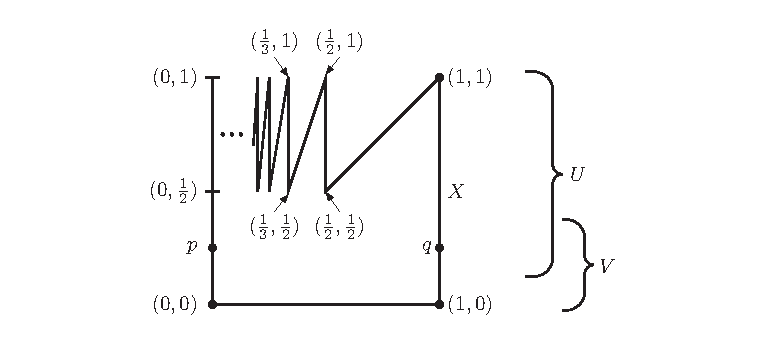
\includegraphics[width=.96\textwidth]{figures/8-13-1.pdf}
\caption*{图 8.13.1}
\end{figure}

再令 $C_n$ 为图 8.13.2 的闭矩形，$D_n=X\cup C_n$。每个 $D_n$ 是多面体，同伦等价于圆，故 $H^1(D_n)\cong\Z$。而 $D_{n+1}$ 是 $D_n$ 的形变收缩核，包含诱导同构。由连续性定理，$\check H^1(X)\cong\varinjlim H^1(D_n)\cong\Z$。\hfill$\square$

\begin{figure}[htbp]\centering
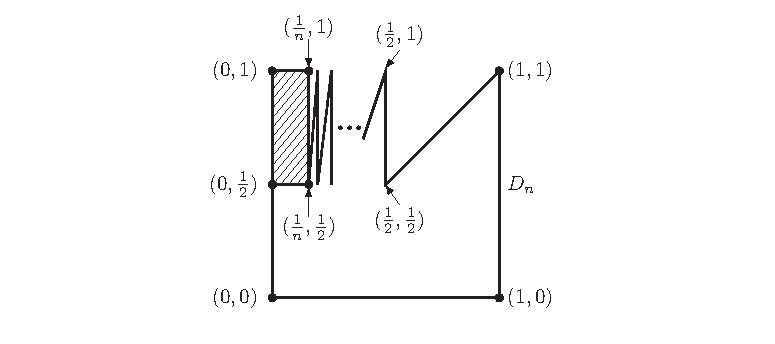
\includegraphics[width=.96\textwidth]{figures/8-13-2.pdf}
\caption*{图 8.13.2}
\end{figure}

这里只初步接触 Čech 上同调。完整理论还需定义连续映射诱导的同态（容易），推广到偶，并验证 Eilenberg--Steenrod 公理（需要一定工作）。参见 [ES52] 第 9、10 章。

\sourcepage{530--531}
\subsection*{习题}
\begin{enumerate}
\item 验证例 8.13.8 的细节。
\item 令 $\mu_n:\Z\to\Z$ 为乘以 $n$。直系统 $\Z\xrightarrow{\mu_2}\Z\xrightarrow{\mu_3}\Z\xrightarrow{\mu_4}\cdots$ 的极限是哪个熟悉的群？
\item 验证定义 Čech 上同调所用的群及同态确实组成直系统。
\item 验证连续性定理证明中引用的加强 Lebesgue 数引理。
\item 设 $X=B^2\times S^1$ 为实心环面，$f:X\to X$ 为图 8.13.3 中的嵌入。令 $X_0=X$，$X_{n+1}=f(X_n)$，$S=\bigcap X_n$，称为\emph{螺线管空间}（solenoid）。(a) 描述 $X_2$；(b) 计算 $\check H^1(S)$。
\begin{figure}[htbp]\centering
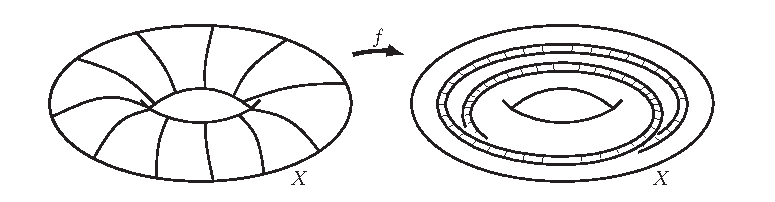
\includegraphics[width=.96\textwidth]{figures/8-13-3.pdf}
\caption*{图 8.13.3}
\end{figure}
\item 令 $\mathcal C$ 为 $X$ 的紧致子空间族，以包含定向。证明它为有向集，令 $G_C=H_i(C)$，结构映射为包含诱导同态，证明
\[H_i(X)\cong\varinjlim_{C\in\mathcal C}H_i(C).\]
这是奇异同调紧支集性质的另一种表述。\translatornote{原文等式左端下标写作 $1$，由所定义直系统应为 $i$。}
\item 对任意集合 $X$，说明如何使其幂集成为有向集。
\end{enumerate}
